%-------------------------------------------------------------------------------
\section{Basic Setup}\label{Setup}
%-------------------------------------------------------------------------------
I now discuss the economics motivating the model analyzed by \citet{Keane.1994} and present their assumptions about functional forms and the distributions of unobservables. Then I turn to the model solution and briefly outline the estimation approach.
%-------------------------------------------------------------------------------
\subsection{Economic Model}
%-------------------------------------------------------------------------------
\citet{Keane.1994} develop a model in which an agent decides among $K$ possible alternatives in each of $T$ (finite) discrete periods of time. Alternatives are defined to be mutually exclusive and $d_k(t) = 1$ indicates that alternative $k$ is chosen at time $t$ and $d_k(t)  = 0$ indicates otherwise. Associated with each choice is an immediate reward $R_k(S(t))$ that is known to the agent at time $t$ but partly unknown from the perspective of periods prior to $t$. The state space $S(t)$ encompasses all the information available to the agent at time $t$ that affects immediate and future rewards.\\\newline
%
Figure \ref{Timing} depicts the timing of events in the model for two generic time periods. At the beginning of period $t$ the agent fully learns about all immediate rewards, chooses one of the alternatives and receives the corresponding payoffs. The state space is then updated according to the agent's state experience and the process is repeated in $t + 1$.
%
\begin{figure}\caption{Timing}\label{Timing}\vspace{1.0cm}\centering

	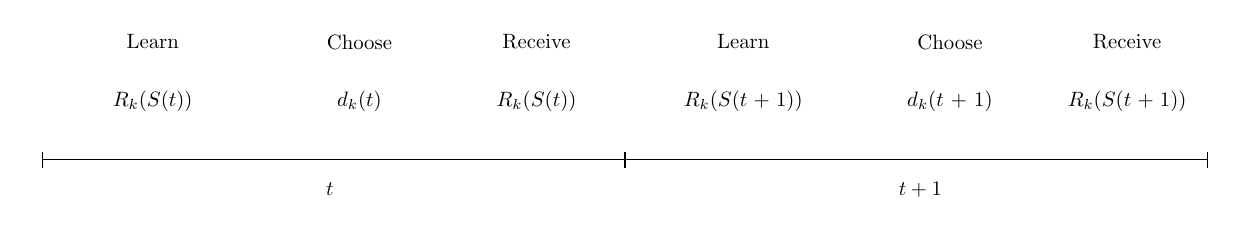
\begin{tikzpicture}[scale=1.0, every node/.style={scale=0.75}]

	\tikzset{
	eqblock/.style={text width=3cm,align=center}
	}

	% Nodes
	\node (left) {};
	\node[node distance=10cm, right of=left] (mid) {};
	\node[node distance=10cm, right of=mid] (right) {};

	\node[node distance=5cm, right of=left, yshift=-.5cm] (t1) {$t$};
	\node[node distance=5cm, right of=mid, yshift=-.5cm] (t2) {$t+1$};

	\node[eqblock, above of=left, xshift=2.0cm] (eq1) {$R_k(S(t))$};
	\node[eqblock, above of=left, xshift=5.5cm] (eq2) {$d_k(t)$};
	\node[eqblock, above of=left, xshift=8.5cm] (eq3) {$R_k(S(t))$};
	\node[eqblock, above of=mid, xshift=2.0cm] (eq4) {$R_k(S(t+1))$};
	\node[eqblock, above of=mid, xshift=5.5cm] (eq6) {$d_k(t+1)$};
	\node[eqblock, above of=mid, xshift=8.5cm] (eq5) {$R_k(S(t+1))$};

	\node[above of=eq1, node distance=1cm] (text2) {Learn};
	\node[above of=eq2, node distance=1cm] (text3) {Choose};
	\node[above of=eq3, node distance=1cm] (text1) {Receive};
	\node[above of=eq4, node distance=1cm] (text4) {Learn};
	\node[above of=eq6, node distance=1cm] (text5) {Choose};
	\node[above of=eq5, node distance=1cm] (text6) {Receive};

	% Lines
	\draw[|-|] (left) -- (mid.center);
	\draw[|-|] (mid.center) -- (right);

	\end{tikzpicture}

\end{figure}
%
Agents are forward looking. Thus, they do not simply choose the alternative with the highest immediate rewards each period. Instead, their objective at any time $\tau$ is to maximize the expected rewards over the remaining time horizon:
%
\begin{align}\label{expectation}
\max_{\{d_k(t)\}_{k \in K}} E\left[ \sum_{\tau = t}^T \delta^{\tau - t} \sum_{k\in K}R_k(\tau)d_k(\tau)\Bigg| S(t)\right].
\end{align}
%
The discount factor $0 > \delta > 1$ captures the agent's preference for immediate over future rewards. Agents maximize equation (\ref{expectation}) by choosing the optimal sequence of alternatives $\{d_k(t)\}_{k \in K}$ for $t = \tau, .., T$.\\\newline

Within this more general model framework, \citet{Keane.1994} then impose additional functional form and distributional assumptions that define their prototypical model of occupational choice.\\\newline
%
Agents live for a total of 40 periods and are risk neutral. Each period, agents choose to work in either of two occupations (k =  1,2), to attend school (k = 3), or to remain at home (k = 4). The immediate reward functions are given by:
%
\begin{align*}
R_1(t) &= w_{1t} =\exp\{\alpha_{10} + \alpha_{11}s_t + \alpha_{12}x_{1t} - \alpha_{13}x^2_{1t} + \alpha_{14}x_{2t} - \alpha_{15}x^2_{2t} + \epsilon_{1t}\}\\
R_2(t) &= w_{2t} =\exp\{\alpha_{20} + \alpha_{21}s_t + \alpha_{22}x_{2t} - \alpha_{23}x^2_{2t} + \alpha_{24}x_{1t} - \alpha_{25}x^2_{1t} + \epsilon_{2t}\}\\
R_3(t) &= \beta_0 - \beta_1 I(s_t \geq 12) - \beta_2(1 - d_3(t -1)) + \epsilon_{3t} \\
R_4(t) &= \gamma_0 + \epsilon_{4t},
\end{align*}
%
where $s_t$ is the number of periods of schooling obtained by the beginning of period $t$, $x_{1t}$ is the number of periods that the agent worked in occupation one by the beginning of period $t$, $x_{2t}$ is the analogously defined level of experience in occupation two, $\alpha_1$ and $\alpha_2$ are parameter vectors associated with the wage functions, $\beta_0$ is the consumption value of schooling, $\beta_1$ is the post-secondary tuition cost of schooling, with $I$ as an indicator function equal to one if the agent completed high school and zero otherwise, $\beta_2$ is an adjustment cost associated with returning to school, $\gamma_0$ is the (mean) value of the non-market alternative. The $\epsilon_{kt}$'s are alternative-specific shocks, to occupational productivity, to the consumption value of schooling, and to the value of non-market time. The productivity and taste shocks follow a four-dimensional multivariate normal distribution with mean zero and covariance matrix $\Sigma = [\sigma_{ij}]$. They collect the parameterization of the reward functions in $\theta = \{\alpha_1, \alpha_2, \beta, \gamma, \Sigma\}$.\\\newline
%
Given the structure of the reward functions and the agent's objective, the state space at time $t$ is $S(t) = \{s_t,x_{1t},x_{2t}, d_3(t - 1),\epsilon_{1t},\epsilon_{2t},\epsilon_{3t},\epsilon_{4t}\}$. It is convenient to denote its observable elements as $\bar{S}(t)$. The elements of $S(t)$ evolve according to:
\begin{align*}
x_{1,t+1}  &= x_{1t} + d_1(t) \\
x_{2,t+1} &= x_{2t} + d_2(t) \\
s_{t+1}   &= s_{t\phantom{2}}    + d_3(t) \\
f(\epsilon_{t+1}\mid S(t), d_k(t)) &= f(\epsilon_{t+1}\mid \bar{S}(t), d_k(t)),
\end{align*}
%
where the last equation reflects the fact that the $\epsilon_{kt}$'s are serially independent. They set the initial conditions as $x_{1t} = x_{2t} = 0$ and $s_0 = 10$. Agents cannot attain more than ten additional years of schooling. Note that all agents start out identically, different choices over the life cycle are simply the cumulative effects of different shocks.
%-------------------------------------------------------------------------------
\subsection{Solution}
%-------------------------------------------------------------------------------
From a mathematical perspective, the model is a finite-horizon dynamic programming (DP) problem under uncertainty that can be solved by backward induction. For the discussion, it is useful to define the value function $V(S(t),t)$ as a shorthand for equation (\ref{expectation}). $V(S(t),t)$ depends on the state space at $t$ and on $t$ itself due to the finiteness of the time horizon and can be written as
%
\begin{align*}
V(S(t),t) = \max_{k \in K}\{V_k(S(t),t)\},
\end{align*}
%
with $V_k(S(t),t)$ as the alternative-specific value function. $V_k(S(t),t)$ obeys the Bellman equation \citep{Bellman.1957} and is thus amenable to a backward induction.
%
\begin{align*}
V_k(S(t),t) = \begin{cases} R_k(S(t)) + \delta E\left[V(S(t + 1), t + 1) \mid S(t), d_k(t) = 1\right] &\qquad\mbox{if } t < T \\
R_k(S(t)) &\qquad\mbox{if } t = T.
\end{cases}
\end{align*}
%
Assuming continued optimal behavior, the expected future value of state $S(t + 1)$ for all $K$ alternatives given today's state $S(t)$ and choice $d_k(t) = 1$, $E\max(S(t + 1))$ for short, can be calculated:
%
\begin{align*}
E\max(S(t + 1)) = E\left[V(S(t + 1), t + 1) \mid S(t), d_k(t) = 1\right].
\end{align*}
%
This requires the evaluation of a $K$ - dimensional integral as future rewards are partly uncertain due to the unknown realizations of the shocks:
%
\begin{align*}
\nonumber E\max(S(t)) =\hspace{11cm}\\
\int_{\epsilon_1(t)}\hdots\int_{\epsilon_K(t)}\max\{R_1(t), \hdots, R_K(t)\}f_{\bs\epsilon}(\epsilon_1(t),\hdots,\epsilon_K(t))d\epsilon_1(t)\hdots d\epsilon_K(t),
\end{align*}
where $f_{\bs\epsilon}$ is the joint density of the uncertain component of the rewards in $t$ not known at $t - 1$. With all ingredients at hand, the solution of the model by backward induction is straightforward.
%-------------------------------------------------------------------------------
\subsection{Estimation}
%-------------------------------------------------------------------------------
Estimation of the parameters of the reward functions $\theta$ is based on a sample of agents whose behavior and state experiences are described by the model. Although all shocks to the rewards are eventually known to the agent, they remain unobserved by the econometrician. So each parameterization induces a different probability distribution over the sequence of observed agent choices and their state experience. Maximum likelihood estimation appraises each candidate parameterization of the model using the likelihood function of the observed sample \citep{Fisher.1922}. Given the serial independence of the shocks, one can compute the likelihood contribution by agent and period. The sample likelihood is then simply the product of the likelihood contributions over all agents and time periods. The agent's choice probabilities are simulated and so one ends up with a simulated maximum likelihood estimator \citep{Manski.1977} minimizing the simulated negative log-likelihood of the observed sample. Additional details about the estimation routine are available in Appendix \ref{Computational Details}.
